\section{Corpus Description} 
The dataset used in this study consists of 130,000 wine 
reviews, sourced from the Wine Enthusiast website 
via Kaggle. Each review includes detailed information 
about the wines, such as the variety, origin, price, 
and the reviewer's evaluation. The primary focus of 
this dataset is the textual description of the wines, 
where reviewers provide sensory insights into the 
wines’ characteristics, such as aroma, flavor, and body.

Not all reviews in the dataset contain complete 
information, and for the purposes of this study, 
reviews missing key data, such as the grape variety, 
were excluded. This cleaned dataset provides a rich 
source of textual data for analyzing how different 
grape varieties are described and for training models 
to classify wines based on these descriptions.

\subsection{Exploratory Data Analysis}
The dataset contains a diverse range of wine varieties, 
with some being more common than others.
\begin{figure*}
    \centering
    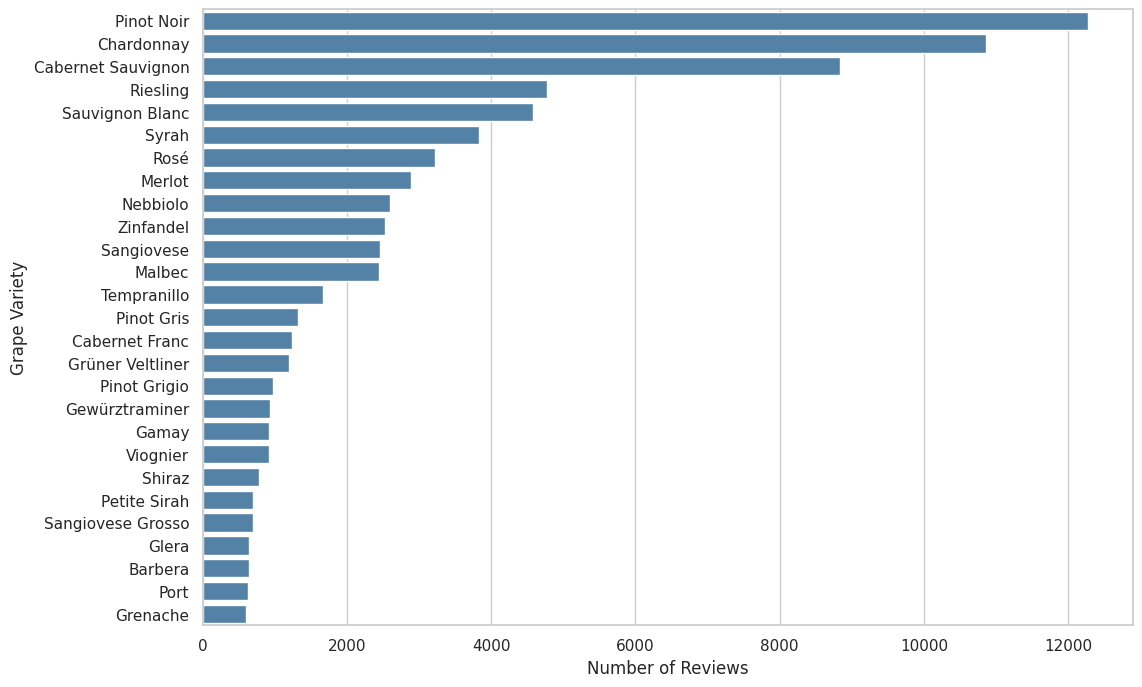
\includegraphics[width=0.8\textwidth]{images/bar_plot_variety_reviews_distribution.png}
    \caption{Most represented grapes varieties in the dataset}
    \label{fig:grape_variety_distribution}
\end{figure*}

To ensure a clearer and more coherent representation 
of wine varieties, a selection was made based on the 
presence of well-defined grape varieties. 
Specifically, varieties labeled as 'Blend' were 
excluded. These varieties represent wines made from 
blends of different grape varieties rather than a 
single variety. Their exclusion was motivated by the 
desire to analyze specific and well-defined grape 
varieties, avoiding the ambiguity introduced by blends.

Additionally, a minimum representation threshold was 
applied to the remaining varieties, ensuring that only 
those with an adequate number of reviews were included 
in the analysis. This approach allowed for a dataset 
focused on clearly identified and sufficiently 
represented wine varieties, facilitating a more 
accurate and meaningful analysis. The selection helped 
avoid distortions due to inadequate representation and 
ensured that the results obtained are based on robust 
and representative data.

As a result of this selection process, the dataset now 
includes \textbf{29} distinct grape varieties, namely 
\textit{Portuguese Red}, \textit{Pinot Gris}, \textit{Riesling}, 
\textit{Pinot Noir}, \textit{Gewürztraminer}, \textit{Cabernet Sauvignon}, 
\textit{Chardonnay}, \textit{Malbec}, \textit{Merlot}, \textit{Gamay}, 
\textit{Sauvignon Blanc}, \textit{Sangiovese}, \textit{Cabernet Franc}, 
\textit{Petite Sirah}, \textit{Rosé}, \textit{Zinfandel}, 
\textit{Grüner Veltliner}, \textit{Viognier}, \textit{Syrah}, 
\textit{Nebbiolo}, \textit{Barbera}, \textit{Portuguese White}, 
\textit{Sangiovese Grosso}, \textit{Shiraz}, \textit{Grenache}, 
\textit{Pinot Grigio}, \textit{Tempranillo}, \textit{Glera}, 
and \textit{Port}. 
After filtering, the cleaned dataset comprises \textbf{85,117} reviews, 
providing a well-defined and comprehensive basis for further analysis.

\subsection{Contamination Removal}
To further refine the dataset, the keyword for each
grape variety was removed from the descriptions. This
was done to eliminate any bias introduced by the
presence of the variety name in the text. By removing
the variety keyword, the analysis can focus solely on
the sensory characteristics and descriptions of the
wines, without being influenced by the specific grape
variety being reviewed.

